\documentclass[
    fontsize      = 11pt,
    paper         = a4,
    twoside       = false,
    parskip       = half,
    pagesize      = false,
]{scrartcl}

\author{Robin Prillwitz}

\usepackage[ngerman]{babel}
\usepackage[iso,german]{isodate}
\date{17 August 2022}

\usepackage{hyphenat}
\hyphenation{Mathe-matik wieder-gewinnen}
\usepackage[babel=true]{csquotes}
\usepackage[protrusion=true,expansion,tracking=true,nopatch=eqnum]{microtype}

\usepackage{amsmath}
\usepackage{amssymb}
\usepackage[locale=DE]{siunitx}

\usepackage[outputdir=./temp/sdu]{minted}

\usepackage{graphicx}
\usepackage{grffile}
\graphicspath{{./img/}}

\usepackage{longtable}
\usepackage{booktabs}

\usepackage[normalem]{ulem}

% % Scale images if necessary, so that they will not overflow the page
% % margins by default, and it is still possible to overwrite the defaults
% % using explicit options in \includegraphics[width, height, ...]{}
% \setkeys{Gin}{width=\maxwidth,height=\maxheight,keepaspectratio}

\usepackage[usenames,dvipsnames,svgnames,table]{xcolor}

\usepackage{tikz}
\usetikzlibrary{patterns}
\usetikzlibrary{calc}
\usetikzlibrary{shapes}
\usetikzlibrary{decorations.markings}
\usetikzlibrary{arrows,automata,backgrounds,petri}
\usepackage[european, betterproportions]{circuitikz}
\usepackage{pgfplots}
\usepackage{pgfplotstable}
\usepackage{pgfgantt}
\usepackage{pgfornament}
\pgfplotsset{
  compat=1.18, % lastest release as of 2022-07-02
}

\usepackage{scrlayer}
\usepackage[]{scrlayer-scrpage}
\ohead{17 August 2022}
\chead{\lowercase{\scshape{sdu}}}
\ihead{Robin Prillwitz}
\ofoot*{\pagemark}
\cfoot*{}

\usepackage[utf8]{inputenc}
\usepackage[T1]{fontenc}
\usepackage{fontspec}
\usepackage{textcomp}

\setsansfont[
    Scale       = MatchLowercase,
    ScaleAgain  = 1.08,
    Ligatures   = TeX
]{Helvetica Neue}

\setmonofont[
    Scale       = MatchLowercase,
    Ligatures   = TeX,
    Contextuals = {Alternate}
]{Fira Code}

\setmainfont[
    Scale       = MatchLowercase,
    UprightFont =  *-Regular,
    BoldFont    =  *-Bold,
    ItalicFont  =  *-It,
    Ligatures   = TeX
]{Minion Pro}

\providecommand{\tightlist}{%
  \setlength{\itemsep}{0pt}\setlength{\parskip}{0pt}}

\usepackage[hidelinks]{hyperref}

\begin{document}

\tableofcontents

\clearpage
\newpage

\hypertarget{intro}{%
\section{Intro}\label{intro}}

\hypertarget{requirements}{%
\subsection{Requirements}\label{requirements}}

\begin{itemize}
\tightlist
\item
  Matlab (with Communications Toolbox)
\item
  Putty / SSH Client
\item
  09:00 to (no later than) 17:00
\end{itemize}

\hypertarget{overview}{%
\subsection{Overview}\label{overview}}

\hypertarget{embodied-ai}{%
\subsubsection{Embodied AI}\label{embodied-ai}}

\clearpage
\newpage

\hypertarget{biological-neurons}{%
\section{Biological-neurons}\label{biological-neurons}}

\hypertarget{neurons}{%
\subsection{Neurons}\label{neurons}}

\begin{itemize}
\tightlist
\item
  \textbf{Dendrite(s)}: Input(s)
\item
  \textbf{Axion}: Output
\item
  \textbf{Soma}: Cell body
\item
  \textbf{Nucleus}: Cell core
\end{itemize}

\emph{Neurons} collect electrical signals to process and transmit to
other \emph{neurons}. \emph{Axon} terminals of one connect to
\emph{dendrites} of other \emph{neurons}. \emph{Synapses} are structures
to connect those electrically/chemically (however no physical connetion
is made).

\hypertarget{synapse}{%
\subsection{Synapse}\label{synapse}}

Electrical signal trasnission through Ion-filled Substrate.

\begin{itemize}
\tightlist
\item
  \textbf{Pre}\emph{synamptic neuron}: Sending Signals from Axiom
\item
  \textbf{Post}\emph{synamptic neuron}: Receiving Signals at the
  Dendrite
\end{itemize}

Voltage changes open Voltage gates from the neural-fluid into the
\emph{presynaptic neuron}. This pulls in Ions from the neuralfluid maing
\emph{vesicles} release realese \emph{neurotransmitteres} into the
\emph{synaptic cleft} to move between the \emph{neurons}. The
\emph{postsynaptic neuron} receives these trasmitteres into receivers
and converts the chemical information to an electrical signal.

\hypertarget{signals}{%
\subsection{Signals}\label{signals}}

\begin{figure}[htp]
\centering
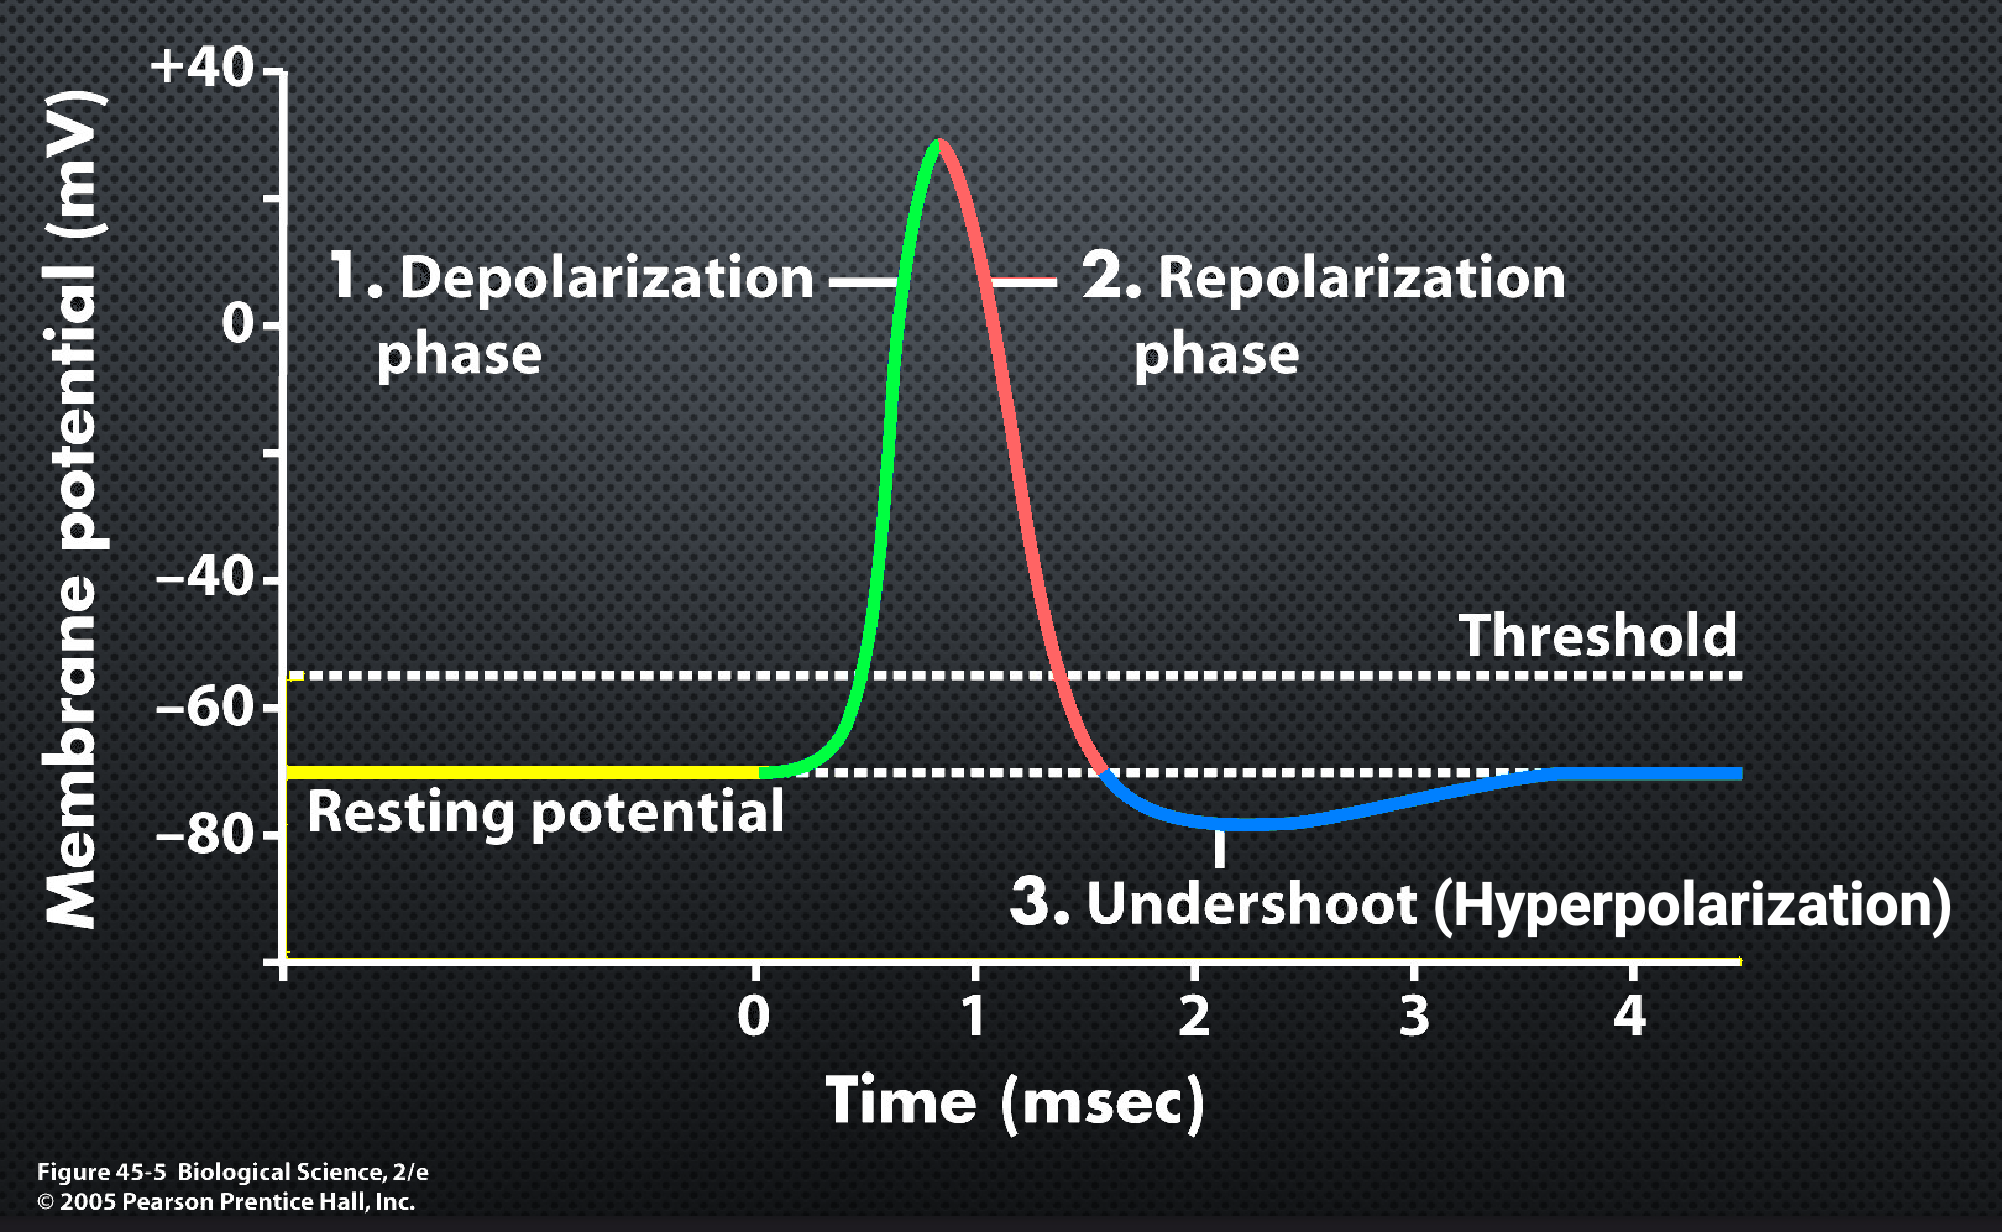
\includegraphics[width=0.5\textwidth]{neuron-spike.png}
\caption{Neuron Spike}
\end{figure}

\begin{itemize}
\tightlist
\item
  \emph{Resting} at \(-70\si{mV}\)
\item
  \emph{Depolarization phase}: Excitation from input signal reaching an
  artificial threshold resulting in a voltage jump (up to
  \(+40\si{mV}\))
\item
  \emph{Repolarization phase}: Return to resting potential
\item
  \emph{Undershoot (Hyperpolarization)} return to resting.
\end{itemize}

All voltages with respect to outside brainfluid.

This process thakes around \(3\si{ms}\ \left( 333.33\si{Hz} \right)\).
The \emph{Myelin Sheaths} decreases performance and throughput aswell.
This is faster due to thight packing and parallel processing.

The spike is seemingly identical between different neurons (same
Amplitude and timeframe).

\hypertarget{resting-membrane-potential-default-state}{%
\subsubsection{Resting membrane potential (default
state)}\label{resting-membrane-potential-default-state}}

Different ion concentration: more negative inside the neuron than
outside. Measurement in reference to outside. Outside: Mostly
\(\mathit{Na}+\) and \(\textit{Cl}-\). Inside: \(\mathit{K}+\) and
\(\mathit{A}-\). Resting voltage sits at around
\(-65\si{mV} \text{ to } -70\si{mV}\).

\hypertarget{de-polarization}{%
\subsubsection{De-polarization}\label{de-polarization}}

Ions flow through the neuron. Signal excites gates. Gates are
ion-specific and only allow certain kinds of ions. These are
\emph{voltage-gates channels}.

Ions like Sodium (\(\mathit{Na}+\)) enter the neuron resulting in a
positive voltage swing up to \(+40\si{mV}\). Once all Sodium gates are
open the threshold is reached. The gates open with very little voltage.

\hypertarget{hyper-polarization}{%
\subsubsection{Hyper-polarization}\label{hyper-polarization}}

Once the voltage between neuron and outside fluid is positive, the
Sodium gates close (as they're voltage controlled). Respectively the
Potassium (\(\mathit{K}+\)) gates open. Positive charge leaves the
neuron making the voltage drop to below the threshold. At resting
potential the Potassium gates close. Due to the delay in closure
undershoot occurs.

\hypertarget{encoding-information}{%
\subsubsection{Encoding Information}\label{encoding-information}}

Information is seemingly encoded in timeing between pulses. Amplitudes
and Durations of spikes are too simmilar between spikes.

\hypertarget{artifical-neruons}{%
\subsection{Artifical Neruons}\label{artifical-neruons}}

\hypertarget{perceptrons}{%
\subsubsection{Perceptrons}\label{perceptrons}}

A simple neural model.

All dendrites \(u_i\) get weighted \(w_i\) and summed resulting in the
activation \(z\). The summation simulates the \emph{soma} core.
\[z = \sum_{i=1}^{n} \omega_i \cdot u_i\]

The threshold and axiom are simulated by an activation function \(\phi\)
resulting in the \emph{perceptrons'} output \(v\). \[v = \phi(z)\]

Activation functions tend to clamp the output in the range of \(-1\) to
\(1\).

An activation function dictates the output space. A heaviside function
can only output a binary result. Functions with infinite range may
diverge. Sigmoid functions can't overflow however the may saturate. The
computataional cost is quite prohibitive.

\hypertarget{hodgkin-huxley-model}{%
\subsubsection{Hodgkin-Huxley Model}\label{hodgkin-huxley-model}}

\begin{figure} [h]
\centering
    \begin{circuitikz}[]
    \draw (0,0) to [short, o-*] ++(0,1);
    \draw (0,7) to [short, *-o] ++(0,1);
    \draw (-3,7) -- (3,7);
    \draw (-3,1) -- (3,1);
    \draw (-3, 1) to[C] ++(0,6);
    \draw (-1, 1) to[C, *-] ++(0,3) to[R, -*] ++(0,3);
    \draw (1, 1) to[C, *-] ++(0,3) to[R, -*] ++(0,3);
    \draw (3, 1) to[C,] ++(0,3) to[R] ++(0,3);
    \end{circuitikz}
\caption{}
\end{figure}

\clearpage
\newpage

\hypertarget{artificial-neural-brains}{%
\section{Artificial neural brains}\label{artificial-neural-brains}}

\hypertarget{braitenberg-vehicles}{%
\subsection{Braitenberg Vehicles}\label{braitenberg-vehicles}}

\begin{itemize}
\tightlist
\item
  \textbf{Ipsilateral}: Connections on same side
\item
  \textbf{Contralateral}: Connections cross sides
\item
  \textbf{Excitatory}: Input Increases \textrightarrow~Output Increases
\item
  \textbf{Inhibitory}: Input Increases \textrightarrow~Output Decreases
\end{itemize}

Vehicle emulates simple \(P\)-type control.

Mathematical model includes:

\begin{itemize}
\tightlist
\item
  \(s_x\): Sensor value
\item
  \(v_x\): Output value
\item
  \(k\): Linear proportional gain
\end{itemize}

Mathematical example implementations:

\begin{itemize}
\tightlist
\item
  \textbf{Ipsilateral}: \(v_{\text{left}} \propto s_{\text{left}}\)
\item
  \textbf{Contralateral}: \(v_{\text{left}} \propto s_{\text{right}}\)
\item
  \textbf{Excitatory}: \(v \propto s\)
\item
  \textbf{Inhibitory}: \(v \propto \frac{1}{s}\)
\end{itemize}

\textbf{Pathplanning}: Finding path from known start to known end
including known obstacles.

Complex behavior emerges by combining multiple weighted control loops
running in parallel.

\clearpage
\newpage

\hypertarget{artificial-learning}{%
\section{Artificial learning}\label{artificial-learning}}

\hypertarget{plasticity}{%
\subsection{Plasticity}\label{plasticity}}

\textbf{Neuroplasticity}: Ability for the brain to re-organize itself in
both \emph{structure} and \emph{function} over time due to external and
internal events. \textbf{Neuroplasticity} is~mechanism behind
``\emph{learning}'' and is happening continuously.

\begin{longtable}[]{@{}ll@{}}
\toprule
\textbf{Structural Plasticity} & ~\textbf{Functional
Plasticity} \\ \addlinespace
\midrule
\endhead
new neural connections & changing existing connections \\ \addlinespace
long-term changes & short term changes \\ \addlinespace
\bottomrule
\end{longtable}

\textbf{Plasticity} happens on all levels from cortical down to the
synaptic level.

\begin{itemize}
\tightlist
\item
  \textbf{cortical}: changing stimulus from limbs triggers different
  existing neurons
\item
  \textbf{synaptic}: changing amount of gates on post-synaptic neurons'
  dendrites
\end{itemize}

\hypertarget{synaptic-strength-in-functional-plasticity}{%
\subsection{\texorpdfstring{\textbf{synaptic strength} in functional
plasticity}{synaptic strength in functional plasticity}}\label{synaptic-strength-in-functional-plasticity}}

\hypertarget{long-term-potentiation-ltp}{%
\subsubsection{\texorpdfstring{Long Term Potentiation
(\emph{LTP})}{Long Term Potentiation (LTP)}}\label{long-term-potentiation-ltp}}

\textbf{HFS}: \(100\) Pulses (over \(1\si{s} \rightarrow 100\si{Hz}\))
as an input to a neuron. The neuron is resting at \(t=0\). The
\textbf{HFS} hits the neuron resulting in an instantaneous output, the
\textbf{LTP}. The neurons output jumps, then receedes and continues to
saturate (Only as long as the \textbf{HFS} is continous.) The
\textbf{synaptic strength} is the chance the output is increased.

A lot of fast input \(\rightarrow\) Big changes and high learning

\textbf{LTP \emph{increases} synaptic strength}

\hypertarget{long-term-depressino-ltd}{%
\subsubsection{\texorpdfstring{Long Term Depressino
(\emph{LTD})}{Long Term Depressino (LTD)}}\label{long-term-depressino-ltd}}

The Inverse, to decrease the \textbf{synaptic strength} an \textbf{LFS}
(\(900\) Pulses \(15\si{min} \rightarrow 1\si{Hz}\)) is sent. The neuron
responsds, dips and saturates in a depression.

Low data \(\rightarrow\) Low learning

\textbf{LTD \emph{decreases} synaptic stregth}

\hypertarget{chemical-basis}{%
\subsubsection{Chemical basis}\label{chemical-basis}}

\textbf{LTP} and \textbf{LTD} result in synapeses by creating or
destroying gates at the pos-synaptic terminal respectively.

\hypertarget{hebbian-learning-model}{%
\subsection{Hebbian learning model}\label{hebbian-learning-model}}

Efficiency describes the likelyhood if a presynaptic neuron spiking and
exciting it's postsynaptic neuron. The likelyhood of the post-synaptic
neuron firing after having been exicted is increased. More firing
together \(\rightarrow\) more likely to fire together in the future.
They spiking is, however, \emph{not necessarily causal}. At high
efficiency the spiking of both neurons are \textbf{temporally
correlated}. The spiking is \textbf{associative} and
\textbf{unsupervised}.

\textbf{Neurons that fire together, wire together.}

\hypertarget{simple-mathematical-model}{%
\subsubsection{Simple mathematical
model}\label{simple-mathematical-model}}

\[\frac{\mathit{d}\omega_1}{\mathit{d}t} = \mu \cdot v \cdot u_1\]

\begin{itemize}
\tightlist
\item
  \(\omega\): dsecribes the synaptic strength / weight
\item
  \(\frac{\mathit{d}\omega_1}{\mathit{d}t}\): (not a derivative), Change
  in synaptic weight
\item
  \(\mu\): Learnig rate (\(\mu \ll 1\) to avoid ``exploding learning
  problem'')
\item
  \(v\): Output of post-synaptic neuron
\item
  \(u_1\): Output of pre-synaptic neuron / input to post-synaptic neuron
\end{itemize}

\[\omega_n = \omega_{n-1} + \frac{\mathit{d}\omega_{n-1}}{\mathit{d}t} = \omega_{n-1} + \mu \cdot v \cdot u_{n-1} \]

\textbf{Problem}: \(\omega_1\) is always increasing, unstable \sout{but
biologically correct}. This is an open control loop.

As this is unsupervised we don't have an error term and can't simply
stop when the model is ``good enough''.

\hypertarget{ltp}{%
\subsubsection{LTP}\label{ltp}}

The further the amount of time between two spikes firing the more the
weight changes. A high \(\delta t\) results in little change, a small
\(\delta t\) results in large changes. At \(\delta t = 0\) maximal
change occurs. The simple model only results in positive change, thus
unstable.

\hypertarget{input-correlation-learning-ico}{%
\subsection{\texorpdfstring{Input correlation learning
(\emph{ICO})}{Input correlation learning (ICO)}}\label{input-correlation-learning-ico}}

Learning rule
\[\frac{\delta w_a}{\delta t} = \eta \cdot f \left( A, t\right) \otimes \frac{\delta f \left( B, t\right) }{\delta t}\]

\begin{itemize}
\tightlist
\item
  \(\eta\): learning rate
\item
  \(f\left( A, t\right) \otimes \frac{\delta f \left( B, t\right) }{\delta t}\):
  Temporal correlation
\item
  \(otimes\): cross correlation
\item
  \(A\): Predictive signal
\item
  \(B\): Reflex signal
\item
  \(Y\): Neuron Ouput
\item
  \(w_a\) weight between \(A\) and \(Y\)
\item
  \(f\) output function of a neuron (including the sigmoid)
\end{itemize}

If we'd like to stop the learning we can assume \(B\) to be constant. We
cannot guarantee \(B \rightarrow 0\) (to stop learning) but we can take
the derivative to stop learning once stimulus ceases change.

This Algorithm \textbf{will converge} to the correct weight.

Output signal is the weighted sum.
\[Y(t) = w_a \cdot f \left( A, t\right) + f \left( B, t\right)\]

\hypertarget{perceptron-learning}{%
\subsubsection{Perceptron learning}\label{perceptron-learning}}

Learning by updating input weights only. Update done using
\textbf{gradient descent}.

Update weight in proportion to contribution to the output. Contribution
is the change in error \(E\) für a given change in \(w\), where the mean
squared error is defined as \[E = \frac{1}{2} \left( t-v\right)^2\]

\begin{itemize}
\tightlist
\item
  \(t\): target output
\item
  \(v\): actual output
\end{itemize}

Determining error requires a known correct output.

\(\rightarrow\) \textbf{supervised learning}

\clearpage
\newpage

\hypertarget{supervised-unsupervised-learning}{%
\section{Supervised \& unsupervised
learning}\label{supervised-unsupervised-learning}}

\hypertarget{non-linear-actiavtion-function}{%
\subsection{Non-linear actiavtion
function}\label{non-linear-actiavtion-function}}

\textbf{Bias} is activation function x-Offset \textbf{Slope} of
activation function is rarely used.

An example sigmoid with \textbf{bias} and \textbf{slope}.
\[v =  \frac{1}{1+e^{-S(z-b)}}\]

where \(b\) is \textbf{bias} and \(S\) the \textbf{slope}. \textbf{Bias}
can be used as a weight.

\begin{align*}
z &= w_1u_1 + w_2u_2 + \ldots + w_nu_n \\
& \rightarrow (z-b) = w_1u_1 + w_2u_2 + \ldots + w_nu_n - b\\
& \rightarrow (z-b) = w_1u_1 + w_2u_2 + \ldots + w_nu_n - (b \cdot -1)\\[2ex]
\rightarrow & (b \cdot -1) \text{ splits to } w_{n+1} \text{ and } u_{n+1}
\end{align*}

This results in an additional weighted bias shifting the activation
function resulting in \[z = \sum_{i=1}^{n+1}\omega_i \cdot u_i\]

Each perceptron can implement one \textbf{deciscion boundary}.
\textbf{Deciscion boundaries} seperate inputs into different classes.
The boundary can be shifted by adapting the weights.

By adding more perceptrons the \textbf{deciscion boundaries} dimension
increases. The boundry of 2 neurons results in one-dimensions. 3 Neurons
create a 2-Dimensional \textbf{deciscion boundary}. More Neurons build
more complex spaces.

\hypertarget{designing-a-network}{%
\subsection{Designing a network}\label{designing-a-network}}

\begin{itemize}
\tightlist
\item
  Defined number of inputs
\item
  Defined number of outputs
\item
  Variable hidden layers
\end{itemize}

Hidden layer depends on linearity of the problem. No general solution to
amount of hidden layers. Strategy of trial and error, start with
\(\approx 100\) layers.

\textbf{Deep Neural Networks}: Depth is defined horizontally.

\hypertarget{convolutional-neural-networks}{%
\subsection{Convolutional neural
networks}\label{convolutional-neural-networks}}

Hereby:

\begin{itemize}
\tightlist
\item
  \(u\): Input
\item
  \(v\) Output
\item
  \(x\) Hidden layer
\item
  \(w\) Weight from \(u\) to \(x\)
\item
  \(y\) Weight from \(x\) to \(v\)
\end{itemize}

One \textbf{Iteration} consists of one forward pass and one backwards
pass. One \textbf{Epoch} consists of \textbf{Iterations} for all Items
in the training set.

\hypertarget{forward-propagation}{%
\subsubsection{Forward propagation}\label{forward-propagation}}

\begin{enumerate}
\def\labelenumi{\arabic{enumi}.}
\tightlist
\item
  Set input
\item
  Calculate for all hidden layers \[x_j = \sum_i u_i w_{ji}\]
\item
  Calculate for all output layers \[v_k = \sum_j x_j w_{kj}\]
\end{enumerate}

\hypertarget{backpropagation}{%
\subsubsection{Backpropagation}\label{backpropagation}}

\begin{enumerate}
\def\labelenumi{\arabic{enumi}.}
\tightlist
\item
  Calculate error gradient for all output neurons
  \[E_k^0 = v_k (1-v_k)(t_k-v_k)\]
\item
  Calculate error gradient for hidden layers
  \[E_j^h = x_j(1-x_j) \sum_k E_K^0 y_{kj}\]
\item
  Update weights for outputs \[y\prime_{kj} = y_{kj} + \mu E_k^0 x_j\]
\item
  Update weights for hidden layers
  \[w\prime_{ji} = w_{ji} + \mu E_j^h u_i\]
\end{enumerate}

\hypertarget{vanishing-gradients}{%
\subsection{Vanishing Gradients}\label{vanishing-gradients}}

With a great amount of layers the impact of early neurons (close to the
input) have less effect on the output error and get changed less
resulting in less learning. A high amount of layers does not guarantee
better network performance.

\textbf{Dropout} randomly disables neurons and stops updating their
weights. This does not guarantee better accuracy only better execution
speed.

This only occurs by learning with backpropagation.

Alternative: \textbf{NEAT} (\emph{Neuroevolution of augmenting
topologies}) using generative algorithms. Possibly (not guaranteed)
better performance to optimize output by chaning the entire networks
structure. Worst execution speed and memory performance.

\hypertarget{trainig-proceedure}{%
\subsection{Trainig proceedure}\label{trainig-proceedure}}

Split trainig dataset into two parts to avoid overfitting. Suggested
split:

\begin{itemize}
\tightlist
\item
  \(70\%\) training data
\item
  \(30\%\) testing data
\end{itemize}

Initilize weights to random values.

\begin{itemize}
\tightlist
\item
  \textbf{Training Datasset}: Adjust weights/learn
\item
  \textbf{Testing Dataset}: Testing final solution
\item
  \textbf{Validation Dataset}: Minimize overfitting
\end{itemize}

Always randomize oder of data for every \textbf{epoch}, as netoworks
easily learn patterns.

More complex splitting algorithms and procesdures:

\begin{itemize}
\tightlist
\item
  \textbf{Monte Carlo corss validation} subsamples data randomly into
  its sets.
\item
  \textbf{K-fold corss validataion} divides data into \(k\) subsets,
  trainig it and removing it after training to repeat with the remaining
  \(k-1\) subsets
\item
  \textbf{Leave-p-out cross validation} \(p\) datasamples, use \(n-p\)
  for training, but test and train \(\frac{n!}{p!\cdot (n-p)!}\) times.
  This presents every datapoint equally often and fairly.
\end{itemize}

\clearpage
\newpage

\hypertarget{questions-answers}{%
\section{Questions \& Answers}\label{questions-answers}}

\hypertarget{biologically-inspired-robotics}{%
\subsection{Biologically inspired
robotics}\label{biologically-inspired-robotics}}

\begin{enumerate}
\def\labelenumi{\arabic{enumi}.}
\item
  \emph{What is biologically-inspired robotics?}

  Using biological systems as inspiration for robotic design.
\item
  \emph{What is biorobotics?}

  Using the biologically inspired robotic system to better understand
  the original biological system.
\item
  \emph{What is the difference between biorobotics and
  biologically-inspired robotics?}

  Biorobotics combines existing biological systems with mechanical
  systems. Biologically-inspired robotics takes inspiration of
  biological systems for robotics without combining the two.
  \textbf{(?)}
\item
  \emph{What is the reality check in biorobotics?}

  Complex biological behaviour doesn't arise from complex systems but
  rather simple, yet dedicated, systems.
\item
  \emph{What is neurorobotics?}

  The study and application of science and technology of embodied,
  autonomous, brain-inspired algorithms.
\item
  \emph{What is a neurorobot? Can you give an example of a neurorobot?}

  A breitenberg vehicle.
\item
  \emph{What is embodied AI?}

  A purpose built mechanical system in conjunction with an AI
  controller.
\item
  \emph{Can you explain the three-layer embodied AI architecture?}

  \begin{itemize}
  \tightlist
  \item
    The controller acting as a supervisor: The brain
  \item
    The mechanical input and outputs: Motors and Sensor
  \item
    The environment
  \end{itemize}
\item
  \emph{Can you give an example of embodied AI in humans/animals? Can
  you give an example of embodied AI in robots?}

  Gas detecting robot inspired by cockroaches.
\item
  \emph{Why is the environment important in embodied AI?}

  An enviornment influences an agent. An agent must overcome external
  influences or take advantage of them. Example: Seagulls in hovering in
  gusts of wind without effort.
\item
  \emph{What are model-based and model-free approaches in biorobotics?
  Can you use both together in one robot? Can you give an example?}

  \begin{itemize}
  \tightlist
  \item
    \textbf{Model based}: A mathematical model defines the entire
    robotic system.
  \item
    \textbf{Model free}: The robot acts according to some defined rules
    but ``figures out'' how to achive it's objective by itself.
  \end{itemize}

  Both appoaches can be used together. A model-based approach defining
  the systems baseline behviour with the model-free system adapting to
  external changes.

  Examples: 3-D Printer controlling it's nozzle temperatur with a model
  (PID Controller) and minimizing motor vibrations using a learning
  algorithm.
\end{enumerate}

\hypertarget{neurons-1}{%
\subsection{Neurons}\label{neurons-1}}

\begin{enumerate}
\def\labelenumi{\arabic{enumi}.}
\item
  \emph{What is a neuron?}

  A biological braincell responsible for processing information.

  It consists of multiple Inputs (\textbf{Dendrites}), one Output
  (\textbf{Axiom}) and it's \textbf{soma} with **nucleus\emph{.}
\item
  \emph{What are the different types of neurons?}

  \begin{itemize}
  \tightlist
  \item
    \textbf{Unipolar}: Inputs, from outside the brain (found in insects)
  \item
    \textbf{Bipolar}: Inputs, from senses (eyes, ears)
  \item
    \textbf{Multipolar}: Within the brain and as outputs to muscles

    \begin{itemize}
    \tightlist
    \item
      \textbf{Pyramidal}: complex though (Cerebrum)
    \item
      \textbf{Purkinje}: reactive action (Cerebellum)
    \end{itemize}
  \end{itemize}
\item
  \emph{How does a neuron work/transmit a signal through itself?}

  Using electrical spikes, presumeably through the spike signal's
  frequency and timing charachteristics, not by it's shape, amplitude or
  phase. \textbf{(?)}
\item
  \emph{How does a neuron forward a signal to other neuron(s)?}

  By using chemical reactions at synapses.
\item
  \emph{What is a synapse?}

  A non-physical connection between two neurons.
\item
  \emph{How does a synapse transmit a signal?}

  The electric signal in the pre-synaptic neuron releases
  neurotransmitters into the synaptic chasm. These travel through the
  brain fluid to the post-synaptic neurons neuroreceptors. If enough
  receptors get stimulated they create an electric spike.
\item
  \emph{What is an action potential?}

  An electrical signal in a neuron.
\item
  \emph{Describe how an action potential is generated.}

  By the neuroreceptors in the post-synaptic neuron.
\item
  \emph{Describe how the different phases of the action potential are
  generated.}

  \begin{itemize}
  \tightlist
  \item
    The \textbf{resting phase} is the default state.
  \item
    The \textbf{depolarization phase} occurs once the Natrium (\(Na+\))
    gates reach a voltage-threshold. A voltage overshoot occurs as
    reactions are not instantenous.
  \item
    The \textbf{repolarization phase} follows showing a decline in
    voltage as the Sodium gates saturate and repell ions, thus allowing
    Potassium (\(K+\)) to enter.
  \item
    The \textbf{hyperpolarization phase} returns to the resting state as
    the voltage reaches an equilibrium.
  \end{itemize}
\item
  \emph{What is resting
  potential/depolarisation/repolarisation/hyperpolarisation? What
  mechanism(s) causes each phase to be generated?}

  \textbf{See above answer}.
\item
  \emph{Why is the resting potential negative?}

  As ions leak through the neurons membrane the neuron takes on a more
  negative charge in respect to the outside fluid.
\item
  \emph{How is information encoded in spikes?}

  Presumeably in its frequency and timing charachteristics.
\item
  \emph{What is a perceptron?}

  A quantized model of a neurons behavior. Consisting of multiple
  weighted inputs getting summed and passed through an activation
  function.
\item
  \emph{What is an activation?}

  The activation describes the weighted sum of the perceptrons inputs.
  \(z = \sum_{i=1}^n \omega_i \cdot u_i\)
\item
  \emph{What is an activation function? Why do we need it/What will
  happen if I don't use it?}

  A mathematical function limiting the perceptrons activation (weighted
  sum) to a knwon output space.
\item
  \emph{What are the different types of activation functions and their
  advantages/drawbacks? Which one will you choose and why?}

  \begin{align*}
   \text{RelU } &= \begin{cases} 0 \text{ for } x < 0\\ x \text{ for } x \geq 0\end{cases}\\[2ex]
   \text{Heaviside } &= \begin{cases} 0 \text{ for } x < 0\\ 0.5 \text{ for } x = 0\\ 1 \text{ for } x > 0\end{cases}\\[2ex]
   \text{Linear } &= x\\
   \text{Sigmoid} &= \frac{1}{1+e^{-x}}
   \end{align*}

  \begin{itemize}
  \tightlist
  \item
    Heaviside limits the output to a binary state, severly reducing
    granularity.
  \item
    Linear and RelU are computationally efficient but may grow
    unbounded.
  \item
    Sigmoids limit the effective range and don't quantize dramatically.
  \end{itemize}
\item
  \emph{Why do we use a sigmoid activation function (think about it from
  both computer implementation and biology perspectives)?}

  It binds the output to a manageable range which avoids overflow and
  offers great precicion using IEE754. It also models neurons' own
  saturation.
\item
  \emph{What is the basic difference between biological neural
  processing and artificial neural processing?}

  Biological neural processing can operate many billions (or more)
  neurons in parallel. Computing with artifical neurons cannot currently
  achieve this.
\item
  \emph{What is a Hodgekin-Huxley model? What
  similarities/dissimilarities does it have with a biological neuron?
  What drawbacks does it have in terms of implementation?}

  An electronic circuit aiming to reproduce neurons' voltage spikes. It
  models different Ion-charges and resistances using batteries and
  resistors acting upon a cpacitor and receiving an external input.

  The model only offers one input. It breaks down with too-high currents
  failing to simulate accordingly. The model only generates spikes and
  it's output is not generally useful for computing.

  It's implementation is computationally incredibly expensive requring
  mutliple equations to be evaluated for every timestep of the voltage
  signal.
\end{enumerate}

\hypertarget{braitenberg-vehicles-1}{%
\subsection{Braitenberg vehicles}\label{braitenberg-vehicles-1}}

\begin{enumerate}
\def\labelenumi{\arabic{enumi}.}
\item
  \emph{What is a Braitenberg vehicle? Can you give an example of one
  and how it behaves?}

  A simple concept of a neurorobot consisting of two powered wheels
  receiving input from two sensors placed at the top left and right of
  the vehicle. The connections between the sensors and wheels dictate
  the vehicles emerging behaviour.

  An agressive vehicle features \textbf{contralateral} and
  \textbf{excitatory} connetions and agressively manouvers towards the
  sensor's gratests stimulus. The \glqq love\grqq vehicle consists of
  \textbf{ipsilateral} and \textbf{inhibitory} connections resulting in
  it seeking the source of gratests stimulus but slowly coming to a halt
  when approaching it.
\item
  \emph{Are there any advantages of using Braitenberg vehicles?}

  Their rather complex behavior emerging from very simplistic rules make
  them computationally trivial.

  They enable emulating behaviors of simple insects.
\end{enumerate}

\hypertarget{learning}{%
\subsection{Learning}\label{learning}}

\begin{enumerate}
\def\labelenumi{\arabic{enumi}.}
\item
  \emph{What is neuroplasticity? What types of neuroplasticity are
  there?}

  Neuroplasticity describes the ability of the brain to re-organize
  itself over time in order to learn. There is \textbf{structural} and
  \textbf{functional} neuroplasticity.
\item
  \emph{What is structural/functional plasticity? What are the
  differences between the two?}

  \begin{itemize}
  \tightlist
  \item
    \textbf{Structural}: Major structural changes over long periods of
    time
  \item
    \textbf{Functional}: Minor adaptions over short periods of time
  \end{itemize}

  There are more biological mechanisms for \textbf{structural} than for
  \textbf{functional} changes.
\item
  \emph{Can you give an example of structural/functional plasticity?}

  \begin{itemize}
  \tightlist
  \item
    \textbf{Structural}:

    \begin{itemize}
    \tightlist
    \item
      Synapses changing in number
    \item
      Synapses receptors changing in density
    \end{itemize}
  \item
    \textbf{Functional}:

    \begin{itemize}
    \tightlist
    \item
      Synapses adjusting their strength (\emph{synaptic plasticity})
    \end{itemize}
  \end{itemize}
\item
  \emph{What is Long Term Potentiation? What is Long Term Depression?
  Can you say something about the chemical process and any changes
  underlying LTP and LDP?}

  \textbf{LTP}: If the synapse is overstimulated for a long period of
  time (many pulses in quick succession, high frequency) the synapse
  will create more neural receptors and thus \glqq strengthen \grqq the
  conection. The \emph{fEPSP} slope increases.

  \textbf{LTD}: If the synapse is, however, understimulated for a long
  time (very few pulses, low frequency), it will reduce the ammount of
  neuroreceptors at the post-synaptic neuron essentially
  \glqq weakening\grqq the conection. The \emph{fEPSP} slope decreases.

  \textbf{(?)}
\item
  \emph{What is Hebbian learning? What are its drawbacks as a model for
  learning?}

  \glqq Neurons that fire together, wire together \grqq

  It describes the likelyhood of a presynaptic neuron spiking and
  exciting it's postsynaptic neuron. The likelyhood of the post-synaptic
  neuron firing after having been exicted is increased. More firing
  together \(\rightarrow\) more likely to fire together in the future.
  They spiking is, however, \textbf{not necessarily causal}. At high
  efficiency the spiking of both neurons are \textbf{temporally
  correlated}. The spiking is \textbf{associative} and
  \textbf{unsupervised}.

  It's model is describes as
  \[\frac{\partial \omega_1}{\partial t} = \mu v u_1\] wherby the
  partial term \(\frac{\partial \omega_1}{\partial t}\) may grow
  unbounded. As this control loop is unsupervised we can't stop the
  model once it's \glqq good enough\grqq.
\item
  \emph{What is Spike-Timing Dependent Plasticity?}

  \textbf{STDP} describes neurons' change in synaptic weight in relation
  to \textbf{LT Potentiation} and \textbf{LT Depression}. This proves a
  biological basis for Hebbian learning, as neurons which have a strong
  temporal correlation have a realtively strong synaptic weight.
\item
  \emph{Do you know other forms of functional plasticity?}

  \begin{itemize}
  \tightlist
  \item
    \textbf{Homosynaptic} plasticity: changes in synapse strength occur
    only at post-synaptic targets that are specifically stimulated by a
    pre-synaptic target.
  \item
    \textbf{Heterosynaptic} plasticity: activity of a third neuron can
    releases chemical neuromodulators that induce changes in synaptic
    strength between two other neurons.
  \item
    \textbf{Non-synaptic} plasticity: intrinsic excitability,
    i.e.~sensitivity to synaptic input, of neurons can be altered and is
    manifested as changes in the firing characteristics of the neuron
    itself.
  \item
    \textbf{Homeostatic} plasticity: capacity of neurons to regulate
    their own excitability relative to network activity, a compensatory
    adjustment that occurs over the timescale of days.
  \end{itemize}
\item
  \emph{What type of plasticity is Hebbian learning (homo-, hetero-,
  non- or homeostatic)?}

  Hebbian learning is \textbf{homosynaptic} plasticity. \textbf{(?)}
\item
  \emph{What is ICO learning? What type of synaptic plasticity is it and
  why? Can you give an example of how ICO learning can be used in
  robots?}

  \textbf{Input correlation learning} (\textbf{ICO}) is
  \textbf{heterosynaptic} plasticity.

  The goal is to detect an event which triggers a reflex signal using a
  predictive signal (without even triggering the reflex). This is
  implemented using the correlation of these two (predictive and reflex
  signal). Implementing this requires a third neuron (one for each input
  and one additional neuron as output), thus \textbf{heterosynapsis} is
  required.

  Example: Detecting obstacles using a camera (predictive input) without
  triggering the bump sensor (reflex input). The robot can learn to
  avoid obstacles by using the camera only.
\item
  \emph{How do perceptrons learn? What is the fundamental difference
  between ICO learning and perceptron learning (think in terms of how
  gradient descent works vs how the ICO learning rule works)?}

  \begin{itemize}
  \tightlist
  \item
    \textbf{ICO} learns by adapting the time between predictive input
    and reflex input (the correlation between those). This process is
    \textbf{unsupervised}.
  \item
    \textbf{perceptrons} learn by adjusting their weight by trying to
    minimize some given error function. This requires an expected output
    and is \textbf{supervised}.
  \end{itemize}
\item
  \emph{What is a Multi-Layer Perceptron (MLP)?}

  An \textbf{MLP} is a neural network. It consists of an input layer, an
  output layer and a defined amount of fully convoluted hidden layers
  inbetween those two.
\item
  \emph{What is the backpropagation algorithm and how does it work? Why
  is it called a gradient descent method?}

  Backpropagation describes the process of changing weights in
  accordance to their respective impact on the output error. An
  errorgradient is calculated for each output neuron and for each hidden
  layer up to the input. Based on this gradient each weight is adjusted
  accordingly.

  The gradient describes an \(n\)-dimensional vector pointing towards
  the steepest decent on the error manifold's surface. Decending this is
  called gradient decent.
\end{enumerate}

\clearpage
\newpage

\hypertarget{robot}{%
\section{Robot}\label{robot}}

\begin{itemize}
\tightlist
\item
  \texttt{192.168.X.1}
\item
  SSID = \texttt{BIOROLE2022\_RobotX}
\item
  PWD = \texttt{BioRoLe2022}
\end{itemize}

Login:

\begin{itemize}
\tightlist
\item
  User: \texttt{pi}
\item
  PWD: \texttt{raspberry}
\end{itemize}

\clearpage
\newpage

\end{document}
